\documentclass{beamer}
\usepackage[utf8]{inputenc}
\usepackage[T1]{fontenc}
\usepackage[brazil]{babel}
\usepackage{graphicx}
\usepackage{booktabs}

\title{Computação Autônoma}
\subtitle{Redes de Computadores I}
\author[Marco Henry, Murilo Neves]{Marco Antônio Cottorello Henry \and Murilo de Souza Neves}
\institute[UEL]{Universidade Estadual de Londrina}
\date{2026}

\AtBeginSection[]
{
  \begin{frame}
    \frametitle{Sumário}
    \tableofcontents[currentsection]
  \end{frame}
}

\usetheme{Szeged}

\begin{document}

  \frame{\titlepage}

  \begin{frame}
    \frametitle{Sumário}
    \tableofcontents
  \end{frame}

  % ===== SEÇÃO 1: HISTÓRICO E DESENVOLVIMENTO =====
  \section{Histórico e Desenvolvimento}

  \begin{frame}
    \frametitle{Motivação: A Crise da Complexidade}
    \begin{columns}
      \column{0.55\textwidth}
      \begin{itemize}
        \item Sistemas modernos: distribuídos, heterogêneos, em nuvem --- componentes de múltiplos fornecedores interagindo em tempo real
        \item \textbf{TCO}: até 80\% do custo de TI em manutenção, não em hardware
        \item \textbf{Erros humanos}: principal causa de falhas em data centers --- complexidade \alert{ultrapassa a capacidade cognitiva humana}
      \end{itemize}

      \column{0.45\textwidth}
      \begin{block}{Manifesto IBM (2001)}
        \textit{``It's Time Systems Take Care of Themselves''}\\[0.3cm]
        Admin define \textbf{o quê} --- sistema decide \textbf{como}\\[0.2cm]
        Inspiração: \textbf{Sistema Nervoso Autônomo (SNA)}
      \end{block}
    \end{columns}
  \end{frame}

  \begin{frame}
    \frametitle{Projetos Precursores}
    \small
    \begin{tabular}{llp{4.8cm}}
      \toprule
      \textbf{Projeto} & \textbf{Ano / Origem} & \textbf{Contribuição principal} \\
      \midrule
      SAS    & 1997 --- DARPA & Roteamento ad-hoc adaptativo em 10.000 nós \\
      DASADA & 2000 --- DARPA & Probes e gauges para monitoramento; precursor direto do MAPE-K \\
      IBM AC & 2001 --- IBM   & Formalização do termo e das 4 propriedades Self-X \\
      SPS    & 2003 --- DARPA & Sistemas auto-regenerativos resistentes a ataques \\
      ANTS   & 2005 --- NASA  & Enxame autônomo para exploração do espaço profundo \\
      \bottomrule
    \end{tabular}
    \vspace{0.3cm}
    \begin{block}{}
      Projetos independentes que convergiram para os mesmos princípios de auto-gestão sem coordenação explícita
    \end{block}
  \end{frame}

  \begin{frame}
    \frametitle{SAS --- Sistema de Consciência Situacional (DARPA, 1997)}
    \begin{columns}
      \column{0.57\textwidth}
      \textbf{Objetivos}
      \begin{itemize}
        \footnotesize
        \item Dispositivos pessoais de comunicação e localização para soldados no campo de batalha
        \item Disseminar relatórios de status autonomamente para até \textbf{10.000} soldados
        \item Latência abaixo de \textbf{200 ms} mesmo sob interferência inimiga
        \item Banda ampla: 20--2.500 MHz, 10 bps a 4 Mbps
      \end{itemize}
      \column{0.43\textwidth}
      \begin{block}{\footnotesize Contribuição para AC}
        \footnotesize
        Primeiro sistema em larga escala de \textbf{roteamento ad-hoc adaptativo} multihop peer-to-peer; demonstrou \textbf{auto-configuração de topologia} dinâmica sob condições adversas
      \end{block}
    \end{columns}
    \vspace{0.15cm}
  \end{frame}

  \begin{frame}
    \frametitle{DASADA --- Montagem Dinâmica para Adaptabilidade (DARPA, 2000)}
    \begin{columns}
      \column{0.57\textwidth}
      \textbf{Objetivos}
      \begin{itemize}
        \footnotesize
        \item Pesquisar e desenvolver tecnologia para sistemas de missão crítica com alta \textbf{confiabilidade, dependabilidade e adaptabilidade}
        \item Tratar a complexidade de sistemas de software distribuídos de grande escala
        \item Objetivo similar ao da iniciativa de Computação Autônoma da IBM
      \end{itemize}
      \column{0.43\textwidth}
      \begin{block}{\footnotesize Contribuição para AC}
        \footnotesize
        Pioneiro na abordagem \textbf{arquitetural} para auto-gestão; introduziu \textbf{probes e gauges} para monitoramento e motor de adaptação baseado em dados --- \alert{precursor direto do MAPE-K}
      \end{block}
    \end{columns}
    \vspace{0.15cm}
  \end{frame}

  \begin{frame}
    \frametitle{SPS --- Sistemas Auto-Regenerativos (DARPA, 2003)}
    \footnotesize
    \textbf{Objetivo:} ``desenvolver tecnologia para sistemas computacionais militares que forneçam funcionalidade crítica em qualquer momento, em face de danos por erros ou ataques'' 
    \vspace{0.15cm}
    \begin{columns}
      \column{0.57\textwidth}
      \textbf{4 aspectos técnicos:}
      \begin{enumerate}
        \footnotesize
        \item Múltiplas versões funcionalmente equivalentes, implementadas diferentemente --- ataque não afeta fração substancial do sistema
        \item Modificações binárias dinâmicas (blocos aleatórios na pilha, endereços de branch variáveis)
        \item Arquitetura de replicação tolerante a intrusões em larga escala
        \item Estimativa de probabilidade de operador malicioso (\textit{insider threat})
      \end{enumerate}
      \column{0.43\textwidth}
      \begin{alertblock}{\footnotesize Contribuição para AC}
        \footnotesize
        Formalizou \textbf{auto-proteção} e \textbf{auto-cura} em sistemas militares; base para sistemas tolerantes a ataques com \textbf{diversidade de implementação}
      \end{alertblock}
    \end{columns}
    \vspace{0.1cm}
  \end{frame}

  \begin{frame}
    \frametitle{Propriedades Self-X}
    \begin{enumerate}

      \item<1-> \textbf{Auto-configuração:} Sistema se instala e ajusta automaticamente segundo metas de alto nível. Um admin especifica o que deseja (ex: servidor web com tempo de resposta < 2s)e não como atingir. Adapta-se a
  plataformas e usuários sem passos manuais.

      \item<2-> \textbf{Auto-cura:} detecta, diagnostica e corrige falhas de hardware e software; tolera falhas e reage aos seus primeiros sinais para garantir continuidade do serviço. Importante corrigir sem prejudicar o sistema.
    \end{enumerate}
  \end{frame}

  \begin{frame}
    \frametitle{Propriedades Self-X (cont.)}
    \begin{enumerate}
      \setcounter{enumi}{2}
       \item<1-> \textbf{Auto-otimização:} busca contínua e \textit{proativa} da eficiência máxima; Redistribui cargas para melhorar o desempenho ou então a \textit{QoS}.
      \item<2-> \textbf{Auto-proteção:} defende contra ataques maliciosos e mudanças prejudiciais; comportamento \textit{proativo} (antecipa brechas) e \textit{reativo} (responde a ameaças) para garantir integridade do sistema.    
      
    \end{enumerate}
    
  \end{frame}

  \begin{frame}
    \frametitle{O Laço de Controle MAPE-K - Imagem}
      \begin{center}
        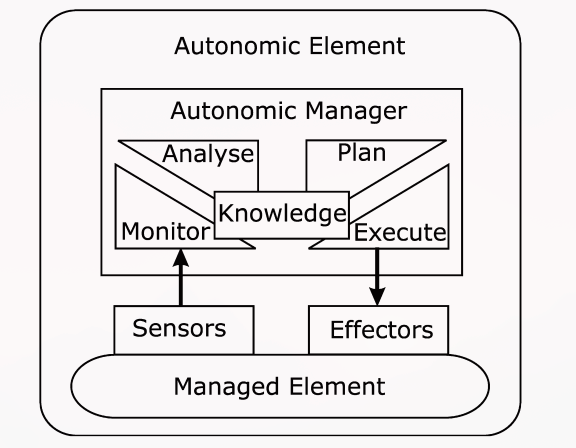
\includegraphics[width=0.75\textwidth]{../texto/mape-k.png}
      \end{center}
  \end{frame}

  \begin{frame}
    \frametitle{Componentes da Arquitetura MAPE-K}
    \begin{itemize}
      \item \textbf{Managed Element:} recurso gerenciado (servidor, rede, aplicação). expõe interface de monitoramento e controle
      \item \textbf{Sensors:} coletam dados do Managed Element e os entregam ao Autonomic Manager 
      \item \textbf{Effectors:} atuadores que aplicam as decisões do Autonomic Manager sobre o Managed Element.
      \item \textbf{Autonomic Manager:} componente central que executa o laço MAPE-K consumindo dados dos sensores e emitindo comandos pelos efetores.
    \end{itemize}
    \vspace{0.2cm}
  \end{frame}

  \begin{frame}
    \frametitle{Autonomic Manager}
    \begin{itemize}

      \item Software configurável via metas de alto nível pelo administrador
      \item Usa dados dos sensores + conhecimento interno para planejar e executar as ações necessárias
      \item O conhecimento interno é
  tipicamente um modelo arquitetural do elemento gerenciado
      
    \end{itemize}
    
  \end{frame}

  \begin{frame}
      \frametitle{Planejamento: Tipos de Políticas}
      \begin{itemize}
        \item \textbf{ECA} (Evento-Condição-Ação)("Se o evento ocorrer, e passar na codição, então faça isso"): diretas e simples; risco de conflito entre múltiplas regras detectável apenas em runtime como conflito por recurso.
        \item \textbf{Objetivo:} define estado desejado; sistema planeja \textit{como} atingi-lo. Mais expressivo, exige maior raciocínio. Quando o estado desejado não é possível ser atingido, sistema não sabe como selecionar o melhor estado indesejado para ficar.
        \item \textbf{Função de Utilidade:} valor numérico por estado; otimiza mesmo quando o estado ideal é inatingível
      \end{itemize}
  \end{frame}

  \begin{frame}
    \frametitle{Monitor: Sensores --- Probes e Gauges}
    \begin{columns}
      \column{0.52\textwidth}
      \textbf{Probes}
      \begin{itemize}
        \footnotesize
        \item Sensores específicos do sistema gerenciado
        \item Extraem dados brutos do \textit{Managed Element}
        \item Especializados na implementação: Java/J2EE, C++, .NET
      \end{itemize}
      \vspace{0.15cm}
      \textbf{Gauges}
      \begin{itemize}
        \footnotesize
        \item Filtram, agregam e processam dados dos probes
        \item Reportam ao Autonomic Manager para planejamento
        \item Especializados no \textbf{problema autônomo} (ex: otimizar disponibilidade de cluster web)
      \end{itemize}
      \column{0.48\textwidth}
      \begin{block}{Correlação Causal}
        \footnotesize
        Gauges determinam \textbf{causa-raiz} correlacionando o instante em que diferentes probes dispararam e fazendo \textit{pattern-matching} nos atributos --- identificam sequência de causalidade da falha
      \end{block}
      \begin{alertblock}{\footnotesize Sensor Distribuído}
        \footnotesize
        Probes e gauges podem estar em \textbf{máquinas diferentes} do elemento gerenciado --- requerem comunicação em rede entre si
      \end{alertblock}
    \end{columns}
  \end{frame}

  \begin{frame}
    \frametitle{Monitor: Monitoramento Passivo e Ativo}
    \begin{columns}
      \column{0.55\textwidth}
      \textbf{Passivo} --- sem instrumentação
      \begin{itemize}
        \footnotesize
        \item \texttt{top}, \texttt{vmstat}: CPU e memória por processo
        \item \texttt{/proc}: pseudo-FS com estado de runtime (Linux)
        \item Equivalentes no Windows 2000/XP
      \end{itemize}
      \vspace{0.2cm}
      \textbf{Ativo} --- com instrumentação
      \begin{itemize}
        \footnotesize
        \item Modificar/adicionar código ao SO ou à aplicação
        \item Capturar chamadas de função ou de sistema
        \item \textbf{ProbeMeister}: insere probes no bytecode Java compilado automaticamente
      \end{itemize}
      \column{0.45\textwidth}
      \begin{block}{QMON (Agarwala et al., 2006)}
        \footnotesize
        Monitor \textbf{autônomo} que adapta sua própria frequência e volume de dados para \textit{minimizar overhead} de monitoramento contínuo e \textit{maximizar utilidade} dos dados coletados
      \end{block}
      \begin{alertblock}{\footnotesize Seleção de Métricas}
        \footnotesize
        Pequeno subconjunto de métricas fornece \textbf{90\% de acurácia} na classificação do estado (Zhang \& Figueiredo, 2006)
      \end{alertblock}
    \end{columns}
  \end{frame}

  \begin{frame}
    \frametitle{Analyse: \textit{Stateless} vs \textit{Stateful}}
    \begin{columns}
      \column{0.5\textwidth}
      \begin{alertblock}{Análise \textit{Stateless}}
        \footnotesize
        Decisão baseada \textbf{apenas} nos dados atuais dos sensores --- sem memória de estado anterior\\[0.2cm]
        Limitação: gestor não reconhece padrões temporais nem tendências --- reage, nunca antecipa
      \end{alertblock}
      \column{0.5\textwidth}
      \begin{block}{Análise \textit{Stateful}}
        \footnotesize
        Autonomic Manager mantém estado do elemento gerenciado, atualizado progressivamente pelos sensores\\[0.2cm]
        Permite \textbf{raciocinar} sobre histórico, detectar anomalias e planejar com contexto completo
      \end{block}
    \end{columns}
    \vspace{0.3cm}
    \begin{block}{}
      \footnotesize
      Abordagem \textit{stateful} requer \textbf{modelo interno} do sistema --- base para a abordagem por modelo arquitetural (\textit{architectural model-driven approach})
    \end{block}
  \end{frame}

  \begin{frame}
    \frametitle{Analyse: Modelo Arquitetural}
    \footnotesize
    \begin{columns}
      \column{0.55\textwidth}
      \begin{itemize}
        \item Autonomic Manager cria e mantém modelo do elemento gerenciado: \textbf{comportamento, requisitos, metas e ambiente operacional}
        \item Modelo atualizado continuamente por dados dos sensores
        \item Adaptações planejadas no modelo \textbf{primeiro} --- sistema real só é alterado se novo estado for válido
        \item Garante \textit{integridade do sistema} após adaptação sem reinicialização
      \end{itemize}
      \column{0.45\textwidth}
      \begin{block}{Componentes e Conectores}
        \footnotesize
        Componentes = tarefas computacionais concorrentes\\
        Conectores = canais de comunicação\\[0.15cm]
        Sem restrição de granularidade: de um servidor Web completo a um único componente de aplicação
      \end{block}
      \begin{alertblock}{Problema: Defasagem}
        \footnotesize
        Delay entre mudança real e atualização do modelo $\rightarrow$ plano executado com base em estado desatualizado
      \end{alertblock}
    \end{columns}
  \end{frame}

  \begin{frame}
    \frametitle{Ciclo MAPE-K: Visão Geral}
    \begin{block}{Ciclo completo}
      \textbf{Monitor} $\rightarrow$ \textbf{Analyse} $\rightarrow$ \textbf{Plan} $\rightarrow$ \textbf{Execute}, sustentado pela base de \textbf{Knowledge} compartilhada entre todas as fases
    \end{block}
    \vspace{0.2cm}
    \begin{itemize}
      \item Monitor coleta via probes/gauges
      \item Analyse raciocina sobre estado atual vs.\ metas --- stateful com modelo arquitetural
      \item Plan define ações: ECA, objetivos ou função de utilidade
      \item Execute aplica via efetores (granularidade fina ou grossa)
    \end{itemize}
  \end{frame}

  
  \begin{frame}
    \frametitle{Base de Conhecimento}
    \begin{itemize}
      \item \textbf{Aprendizado por Reforço:} aprende políticas por tentativa e erro, vendo as consequências das ações; não exige modelo explícito do sistema gerenciado. 
      \item \textbf{Redes Bayesianas:} decisão probabilística sob incerteza; seleção de algoritmos sensível a custo
      \item \textbf{Modelos Arquiteturais:} verifica validade das mudanças \textit{antes} de executar no sistema real
    \end{itemize}
  \end{frame}

  \section{Sistemas Multitier e Graus de Autonomia}

  \begin{frame}
      \frametitle{Sistemas Multitier Autônomos}
      \begin{columns}
        \column{0.52\textwidth}
        \begin{itemize}
          \item E-commerce típico: 3 tiers independentes
          \begin{itemize}
            \item Tier web: Apache
            \item Tier aplicação: J2EE
            \item Tier banco de dados: DB2/Oracle
          \end{itemize}
          \item Cada tier implementa \textbf{seu próprio MAPE-K}
          \item Problema: alocação entre tiers é \textit{acoplada} --- BD não pode ser replicado sob demanda
        \end{itemize}
        \column{0.48\textwidth}
        \begin{block}{Solução}
          Gerenciadores autônomos precisam estar cientes do ambiente, incluindo \textbf{outros elementos autônomos} na rede
        \end{block}
        \vspace{0.3cm}
        \begin{alertblock}{Resultado}
          Redistribuição dinâmica de recursos entre tiers mantém desempenho total mesmo sob carga variável
        \end{alertblock}
      \end{columns}
  \end{frame}

  
  \begin{frame}
    \frametitle{Graus de Autonomicidade: Modelo IBM}
    \footnotesize
    \begin{tabular}{cp{1.8cm}p{5.8cm}}
      \toprule
      \textbf{Nível} & \textbf{Nome} & \textbf{Descrição} \\
      \midrule
      1 & Básico     & Staff qualificado gerencia manualmente com ferramentas de monitoramento \\
      2 & Gerenciado & Ferramentas coletam informações de forma inteligente, reduzem carga administrativa \\
      3 & Preditivo  & Monitoramento reconhece padrões de comportamento e \textit{sugere} ações ao staff \\
      4 & Adaptativo & Sistema age com intervenção humana mínima; ajusta para cumprir os acordos em níveis de serviço \\
      5 & Autônomo   & Componentes gerenciados dinamicamente por regras de negócio --- plena autonomia \\
      \bottomrule
    \end{tabular}
    \vspace{0.2cm}
    \begin{block}{}
      IBM estima que a maioria dos sistemas de TI atuais está nos níveis 1--2
    \end{block}
  \end{frame}


  % ===== SEÇÃO 3: APLICAÇÕES =====
  \section{Aplicações}

  \begin{frame}
    \frametitle{Cooperação entre Gerenciadores Autônomos}
    \begin{itemize}
      \item Elementos autônomos podem \textbf{cooperar} para atingir objetivo comum (ex: minimizar tempo de resposta total do cluster)
      \item \textbf{Abordagem multi-agente:} cada gerenciador é um agente; comportamento global \textit{emerge} da interação local
      \item \textbf{Abordagem hierárquica:} estruturação em níveis de abstração --- alternativa à cooperação peer-to-peer
      \item Desafio central: garantir que objetivos locais de cada agente resultem no \textbf{objetivo global} sendo atingido
    \end{itemize}
    \vspace{0.2cm}
    \begin{block}{Objetivo da Cooperação}
      Design proposital de protocolos de interação para que resultado desejável e previsível \textit{emerge} em nível superior sem coordenação central explícita
    \end{block}
  \end{frame}

  \begin{frame}
    \frametitle{Emergência Engenheirada}
    \begin{columns}
      \column{0.55\textwidth}
      \footnotesize
      \begin{itemize}
        \item \textbf{Definição:} ``design proposital de protocolos de interação de modo que resultado previsível e desejável é alcançado em nível superior'' (Anthony, 2006)
        \item Inspiração: colônias de insetos --- regras locais simples geram comportamento global complexo e robusto
        \item Cada nó opera com \textbf{informação local limitada}; nenhum nó conhece o estado global
        \item Contraste com algoritmo distribuído clássico: sem ACKs obrigatórios, sem ordenação rígida de eventos
      \end{itemize}
      \column{0.45\textwidth}
      \begin{block}{Características}
        \footnotesize
        \begin{itemize}
          \item Escala
          \item Robustez
          \item Estabilidade
          \item Sem ponto único de falha
        \end{itemize}
      \end{block}
      \begin{alertblock}{Desafio}
        \footnotesize
        Garantir que o comportamento emergente seja o \textit{desejado} --- sistemas naturais não garantem isso
      \end{alertblock}
    \end{columns}
  \end{frame}

  \begin{frame}
    \frametitle{Aplicação Clássica: NASA ANTS --- Contexto}
    \begin{itemize}
      \item 1.000 nanoespaçonaves (\textless{}1 kg) no cinturão de asteróides
      \item 60--70\% de perda esperada ao entrar no cinturão
      \item Atraso de comunicação com Terra inviabiliza controle humano em tempo real
      \item Papéis distribuídos: trabalhadores, coordenadores, mensageiros
    \end{itemize}
  \end{frame}

  \begin{frame}
    \frametitle{Aplicação Clássica: NASA ANTS --- Self-X}
    \begin{itemize}
      \item \textbf{Auto-cura:} sobreviventes redistribuem papéis das naves perdidas automaticamente
      \item \textbf{Auto-config.:} cada nave determina posição na frota e rotas com vizinhos disponíveis
      \item \textbf{Auto-otimiz.:} prioriza asteróides com base nos dados já coletados
      \item \textbf{Auto-proteção:} evita colisões; gerencia consumo de energia das velas solares
    \end{itemize}
    \vspace{0.3cm}
    \begin{block}{}
      MAPE-K distribuído: cada nave executa ciclo local; comportamento global coerente emerge do enxame
    \end{block}
  \end{frame}

  \begin{frame}
    \frametitle{Aplicação Clássica: IBM \textit{Project eLiza}}
    \begin{itemize}
      \item Maior foco individual de investimento da divisão de servidores IBM --- linha \textit{eServer} (zSeries, pSeries, iSeries, xSeries)
      \item Espinha dorsal de operações bancárias, de telecomunicações e governamentais globais
      \item \textbf{Auto-config.:} hardware e middleware se reconfiguram na inicialização e em runtime sem intervenção do operador
      \item \textbf{Auto-otimização:} \textit{Intelligent Resource Director} (IRD) redistribui cargas entre partições lógicas (LPARs) para maximizar throughput e cumprir SLAs
    \end{itemize}
  \end{frame}

  \begin{frame}
    \frametitle{Aplicação Clássica: IBM \textit{Project eLiza} (cont.)}
    \begin{itemize}
      \item \textbf{Auto-cura:} \textit{System Automation for OS/390} detecta falhas em aplicações e aciona recuperação automática --- inicia, para, monitora e recupera serviços sem humano
      \item \textbf{Auto-proteção:} detecção de intrusão e isolamento de falhas integrados diretamente ao SO
    \end{itemize}
    \vspace{0.4cm}
    \begin{alertblock}{}
      Provou que Self-X é viável em sistemas de missão crítica em produção real
    \end{alertblock}
  \end{frame}


  \begin{frame}
    \frametitle{Orquestração e Auto-scaling em Nuvem}
    \begin{columns}
      \column{1\textwidth}
      A Computação Autônoma atua como o motor de orquestração essencial para manter a viabilidade econômica dos provedores modernos.
      \begin{itemize}
        \item{\textbf{Auto-otimização:}}Provisionamento dinâmico (auto-scaling) baseado em métricas de CPU e latência em tempo real. Economizando energia e custo.
        \item{\textbf{Eficiência Energética:}} Consolidação de cargas de trabalho e desligamento de recursos ociosos.
        \item{\textbf{Resiliência:}}Detecção de degradação e migração automática de VMs sem interrupção de serviço. Por meio de migração automática de VMs e reconfiguração de balanceadores.
      \end{itemize}
    \end{columns}
  \end{frame}

  \begin{frame}
    \frametitle{Orquestração e Auto-scaling em Nuvem}
    \begin{figure}
      \centering
      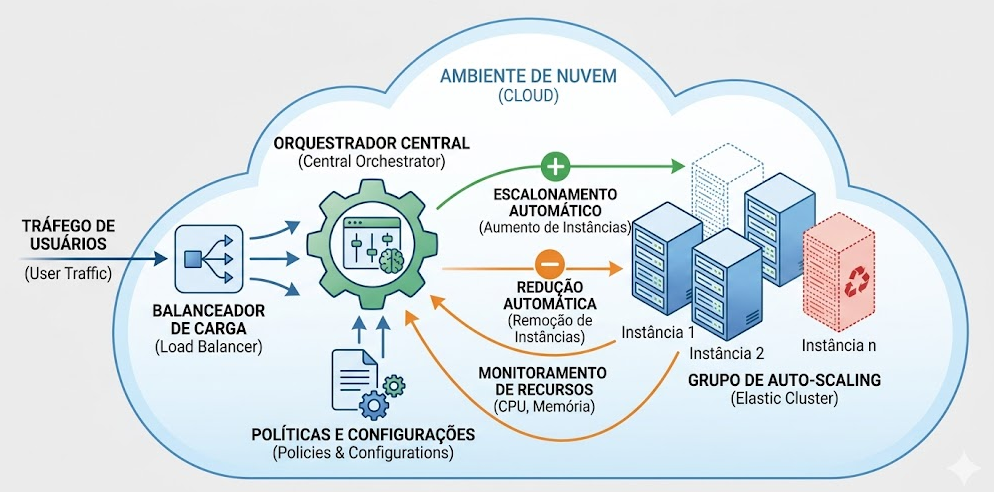
\includegraphics[scale=0.3]{./images/orquestracao_nuvem.png}
      \caption{Funcionamento da orquestração em nuvem}
    \end{figure}
  \end{frame}

  \begin{frame}
    \frametitle{Sistemas Pervasivos e IoT}
    \begin{itemize}
      \item Desafio: heterogeneidade + volatilidade + recursos limitados.
      \item Auto-configuração: dispositivos plug-and-play em Smart Cities e Smart Grids. Descobrem vizinhos e registram serviços automaticamente.
      \item Auto-proteção: detecção de tráfego anômalo (DDoS, intrusões) e quarentena automática de dispositivos comprometidos.
      \item Sem autonomia, o custo de configurar milhões de sensores seria proibitivo.
    \end{itemize}
  \end{frame}

  % ===== SEÇÃO 4: ESTADO DA ARTE =====
  \section{Estado da Arte}

  \begin{frame}
    \frametitle{Estado da Arte: Mudança de Paradigma}
    A pesquisa não busca mais justificar a autonomia, mas refinar o MAPE-K e resolver suas limitações.

    Principal mudança no método foi sair de regras estáticas para a autonomia preditiva com IA/ML.
    \begin{itemize}
      \item Aprendizado por Reforço e Redes Neurais Profundas substituem políticas estáticas se-então.
      \item O sistema aprende políticas ótimas por tentativa e erro ou via dados históricos.
    \end{itemize}
  \end{frame}

  \begin{frame}
    \frametitle{Paradigmas Industriais Consolidados}
    AIOps (Artificial Intelligence for IT Operations)
    \begin{itemize}
      \item Estado da arte em auto-cura e auto-otimização de data centers.
      \item Ingere terabytes de logs/métricas e antecipa falhas horas antes de ocorrerem.
    \end{itemize}
    Orquestração Cloud-Native \& Service Mesh
    \begin{itemize}
      \item Microsserviços adotam Self-X de forma nativa.
      \item Kubernetes + Service Mesh $\rightarrow$ auto-configuração e auto-cura em milissegundos.
    \end{itemize}
  \end{frame}

  \begin{frame}
    \frametitle{Lacunas e Desafios em Aberto}
    \begin{enumerate}
      \item Verificação Formal e Estabilidade\\
      Problema da ``caixa-preta'' do ML $\rightarrow$ necessidade de provar matematicamente a corretude.

      \item Interoperabilidade \& Sistemas Multi-agente\\
      Soluções atuais vivem em silos; falta padronização para troca de conhecimento entre gerentes autônomos.

      \item Tradução de Políticas de Alto Nível\\
      Converter metas de negócio (``maximizar lucro minimizando latência'') em ações operacionais ainda exige especialista humano.
    \end{enumerate}

    Fronteira atual: tornar a autonomia verificável, interpretável e interoperável.
  \end{frame}

  % ===== SEÇÃO 5: CONCLUSÃO =====
  \section{Conclusão}

  \begin{frame}
    \frametitle{Conclusão}
    \begin{itemize}
      \item A escalabilidade da TI moderna não pode mais ser dissociada da automação de sua gestão.
      \item A capacidade cognitiva humana é o principal limitador das infraestruturas contemporâneas.
      \item A ``crise da complexidade'' é o desafio central. A Computação Autônoma é a resposta.
      \item As propriedades Self-X, sustentadas pelo MAPE-K, viabilizam Cloud, IoT e sistemas pervasivos não apenas tecnicamente, mas economicamente (redução de TCO + cumprimento de SLAs).
    \end{itemize}
  \end{frame}

  \begin{frame}
    \frametitle{Conclusão}
    A transição de sistemas que auxiliam decisões $\rightarrow$ para sistemas que agem sozinhos ainda esbarra em:
    \begin{itemize}
      \item Interoperabilidade entre fornecedores
      \item Confiança dos administradores
      \item Estabilidade formal dos algoritmos
    \end{itemize}

    Em uma era de trilhões de dispositivos, autonomia deixa de ser diferencial e passa a ser requisito mandatório.
  \end{frame}

  \begin{frame}
    \frametitle{Referências Principais}
    \begin{itemize}
      \item IBM (2001). \textit{Autonomic Computing: An Architectural Blueprint}
      \item Kephart \& Chess (2003). \textit{The Vision of Autonomic Computing}. IEEE Computer
      \item Sterritt (2005). \textit{Autonomic Computing}. Innovations in Systems and Software Engineering
      \item Lalanda et al.\ (2013). \textit{Autonomic Computing: Principles, Design and Implementation}
      \item Ganek \& Corbi (2003). \textit{The dawning of the autonomic computing era}. IBM Systems Journal
      \item Truszkowski et al.\ (2004). \textit{Autonomous and Autonomic Systems}
    \end{itemize}
    \vspace{0.4cm}
    \centering
    \Large \textbf{Obrigado!}
  \end{frame}

  % ===== PERGUNTAS E RESPOSTAS =====
  \section*{Perguntas e Respostas}

  \begin{frame}
    \frametitle{P\&R 1: O que motivou a Computação Autônoma?}
    \begin{alertblock}{Pergunta}
      Qual foi a principal motivação para o surgimento da Computação Autônoma e qual foi o papel da IBM?
    \end{alertblock}
    \begin{block}{Resposta}
      A ``crise da complexidade'': TCO com até 80\% em manutenção e erros humanos como principal causa de falhas em data centers. Em 2001, a IBM publicou manifesto propondo sistemas auto-gerenciáveis inspirados no Sistema Nervoso Autônomo (SNA) --- administrador define metas de alto nível, sistema decide como atingi-las.
    \end{block}
  \end{frame}

  \begin{frame}
    \frametitle{P\&R 2: Quais são as propriedades Self-X?}
    \begin{alertblock}{Pergunta}
      Quais são as 4 propriedades Self-X e como elas se complementam?
    \end{alertblock}
    \begin{block}{Resposta}
      \footnotesize
      \begin{itemize}
        \item \textbf{Auto-config.:} sistema se instala e ajusta sem passos manuais
        \item \textbf{Auto-cura:} detecta, diagnostica e corrige falhas de HW/SW
        \item \textbf{Auto-otimização:} redistribui recursos \textit{proativamente} para cumprir SLAs
        \item \textbf{Auto-proteção:} defende contra ataques --- proativa e reativa
      \end{itemize}
    \end{block}
  \end{frame}

  \begin{frame}
    \frametitle{P\&R 3: Como funciona o ciclo MAPE-K?}
    \begin{alertblock}{Pergunta}
      Descreva o ciclo MAPE-K e o papel da base de Conhecimento.
    \end{alertblock}
    \begin{block}{Resposta}
      \footnotesize
      \textbf{Monitor} coleta $\rightarrow$ \textbf{Analyse} identifica desvios vs.\ metas $\rightarrow$ \textbf{Plan} define ações $\rightarrow$ \textbf{Execute} aplica via efetores.\\[0.2cm]
      \textbf{Knowledge} sustenta todas as fases: políticas, histórico e modelos arquiteturais --- valida mudanças antes de executar no sistema real.
    \end{block}
  \end{frame}

  \begin{frame}
    \frametitle{P\&R 4: Computação Autônoma em Cloud e IoT}
    \begin{alertblock}{Pergunta}
      Como a Computação Autônoma se manifesta em Cloud Computing e IoT?
    \end{alertblock}
    \begin{block}{Resposta}
      \footnotesize
      \textbf{Cloud:} auto-scaling por MAPE-K; falha de nó $\rightarrow$ migração automática de VMs.\\[0.15cm]
      \textbf{IoT:} sensores com \textit{plug-and-play}; dispositivos comprometidos isolados em quarentena automaticamente.
    \end{block}
  \end{frame}

  \begin{frame}
    \frametitle{P\&R 5: Desafios para Adoção Plena}
    \begin{alertblock}{Pergunta}
      Quais são os principais desafios que impedem a adoção plena da Computação Autônoma?
    \end{alertblock}
    \begin{block}{Resposta}
      \footnotesize
      \begin{enumerate}
        \item \textbf{Verificação Formal:} ML é ``caixa-preta'' --- difícil provar corretude matematicamente
        \item \textbf{Interoperabilidade:} soluções em silos; falta protocolo para troca de Knowledge entre gerentes
        \item \textbf{Tradução de Políticas:} metas de negócio ainda exigem especialista para mapear em config.\ operacional
      \end{enumerate}
    \end{block}
  \end{frame}

\end{document}
